% Options for packages loaded elsewhere
\PassOptionsToPackage{unicode}{hyperref}
\PassOptionsToPackage{hyphens}{url}
%
\documentclass[
]{article}
\usepackage{amsmath,amssymb}
\usepackage{iftex}
\ifPDFTeX
  \usepackage[T1]{fontenc}
  \usepackage[utf8]{inputenc}
  \usepackage{textcomp} % provide euro and other symbols
\else % if luatex or xetex
  \usepackage{unicode-math} % this also loads fontspec
  \defaultfontfeatures{Scale=MatchLowercase}
  \defaultfontfeatures[\rmfamily]{Ligatures=TeX,Scale=1}
\fi
\usepackage{lmodern}
\ifPDFTeX\else
  % xetex/luatex font selection
  \setmainfont[]{DejaVu Serif}
\fi
% Use upquote if available, for straight quotes in verbatim environments
\IfFileExists{upquote.sty}{\usepackage{upquote}}{}
\IfFileExists{microtype.sty}{% use microtype if available
  \usepackage[]{microtype}
  \UseMicrotypeSet[protrusion]{basicmath} % disable protrusion for tt fonts
}{}
\makeatletter
\@ifundefined{KOMAClassName}{% if non-KOMA class
  \IfFileExists{parskip.sty}{%
    \usepackage{parskip}
  }{% else
    \setlength{\parindent}{0pt}
    \setlength{\parskip}{6pt plus 2pt minus 1pt}}
}{% if KOMA class
  \KOMAoptions{parskip=half}}
\makeatother
\usepackage{xcolor}
\usepackage[margin=2.5cm]{geometry}
\usepackage{longtable,booktabs,array}
\usepackage{calc} % for calculating minipage widths
% Correct order of tables after \paragraph or \subparagraph
\usepackage{etoolbox}
\makeatletter
\patchcmd\longtable{\par}{\if@noskipsec\mbox{}\fi\par}{}{}
\makeatother
% Allow footnotes in longtable head/foot
\IfFileExists{footnotehyper.sty}{\usepackage{footnotehyper}}{\usepackage{footnote}}
\makesavenoteenv{longtable}
\usepackage{graphicx}
\makeatletter
\def\maxwidth{\ifdim\Gin@nat@width>\linewidth\linewidth\else\Gin@nat@width\fi}
\def\maxheight{\ifdim\Gin@nat@height>\textheight\textheight\else\Gin@nat@height\fi}
\makeatother
% Scale images if necessary, so that they will not overflow the page
% margins by default, and it is still possible to overwrite the defaults
% using explicit options in \includegraphics[width, height, ...]{}
\setkeys{Gin}{width=\maxwidth,height=\maxheight,keepaspectratio}
% Set default figure placement to htbp
\makeatletter
\def\fps@figure{htbp}
\makeatother
\setlength{\emergencystretch}{3em} % prevent overfull lines
\providecommand{\tightlist}{%
  \setlength{\itemsep}{0pt}\setlength{\parskip}{0pt}}
\setcounter{secnumdepth}{-\maxdimen} % remove section numbering
\ifLuaTeX
\usepackage[bidi=basic]{babel}
\else
\usepackage[bidi=default]{babel}
\fi
\babelprovide[main,import]{russian}
\ifPDFTeX
\else
\babelfont{rm}[]{DejaVu Serif}
\fi
% get rid of language-specific shorthands (see #6817):
\let\LanguageShortHands\languageshorthands
\def\languageshorthands#1{}
\ifLuaTeX
  \usepackage{selnolig}  % disable illegal ligatures
\fi
\usepackage{bookmark}
\IfFileExists{xurl.sty}{\usepackage{xurl}}{} % add URL line breaks if available
\urlstyle{same}
\hypersetup{
  pdflang={ru},
  hidelinks,
  pdfcreator={LaTeX via pandoc}}

\author{}
\date{}

\begin{document}

\section{Влияние вязкоупругой релаксации на чувствительность
термомеханического состояния пресноводного льда к геометрии воздушной
поры при случайном температурном
воздействии}\label{ux432ux43bux438ux44fux43dux438ux435-ux432ux44fux437ux43aux43eux443ux43fux440ux443ux433ux43eux439-ux440ux435ux43bux430ux43aux441ux430ux446ux438ux438-ux43dux430-ux447ux443ux432ux441ux442ux432ux438ux442ux435ux43bux44cux43dux43eux441ux442ux44c-ux442ux435ux440ux43cux43eux43cux435ux445ux430ux43dux438ux447ux435ux441ux43aux43eux433ux43e-ux441ux43eux441ux442ux43eux44fux43dux438ux44f-ux43fux440ux435ux441ux43dux43eux432ux43eux434ux43dux43eux433ux43e-ux43bux44cux434ux430-ux43a-ux433ux435ux43eux43cux435ux442ux440ux438ux438-ux432ux43eux437ux434ux443ux448ux43dux43eux439-ux43fux43eux440ux44b-ux43fux440ux438-ux441ux43bux443ux447ux430ux439ux43dux43eux43c-ux442ux435ux43cux43fux435ux440ux430ux442ux443ux440ux43dux43eux43c-ux432ux43eux437ux434ux435ux439ux441ux442ux432ux438ux438}

\emph{Рабочая редакция 0.1 --- 22 октября 2026 г. Текст для научного
обсуждения, не для подачи в редакцию.}

\textbf{Авторы, аффилиации, УДК и сведения о финансировании:} будут
утверждены в следующей редакции.

\subsection{Аннотация}\label{ux430ux43dux43dux43eux442ux430ux446ux438ux44f}

Рассматривается трёхмерная нестационарная термомеханическая задача для
ограниченного фрагмента пресноводного льда со сферической воздушной
порой, расположенной вблизи охлаждаемой поверхности. Целью исследования
является количественная оценка того, как малые изменения радиуса,
вертикального положения и осесимметричной несферичности поры влияют на
математическое ожидание и дисперсию интегрального показателя
растягивающего напряжённого состояния при случайном охлаждении.
Использована односторонне связанная постановка: нестационарная
теплопроводность с конвективным теплообменом на верхней грани,
квазистатическое равновесие и модель с упругой, запаздывающей и вязкой
составляющими деформации. Мгновенный модуль Юнга зависит от температуры
по нормированному относительному закону. Показатель состояния
определяется сглаженной спектральной функцией трёх главных напряжений,
осреднённой по фиксированной окрестности полости и времени наблюдения.
Трёхмерная дискретизация использует квадратичные тетраэдральные
элементы; геометрические производные определяются центральными
разностями, а вероятностные моменты --- квадратурой Гаусса--Эрмита. Для
основной сетки получены производные математического ожидания по радиусу,
вертикальному смещению и гармонике \(Y_{20}\), равные соответственно
\(0.1003537\), \(-0.0005272\) и \(-0.0270151\) м⁻¹; производные
дисперсии составили \(2.01429\cdot10^{-4}\), \(-1.07481\cdot10^{-6}\) и
\(-5.46217\cdot10^{-5}\) м⁻¹. Проверены сгущение сеток, шаг
геометрического возмущения, временная дискретизация и повышение порядка
стохастической квадратуры. По трём геометрическим модам построены
осесимметричные проекции поверхностной чувствительности, выявляющие
различие полярных и экваториальной областей. Обсуждены границы
применимости результатов, в том числе различия между пространственной и
временной стабилизацией, условность используемого материала и
необходимость последующей проверки полным сопряжённым градиентом формы.
Полученные результаты предназначены для интерпретации малых
геометрических вариаций при фиксированной вероятностной модели, а не для
непосредственного прогноза растрескивания или прочности конкретного
ледяного образца.

\textbf{Ключевые слова:} пресноводный лёд; сферическая пора;
термомеханика; вязкоупругость; чувствительность формы; стохастическое
охлаждение; метод конечных элементов; сферические гармоники;
математическое ожидание; дисперсия; квадратура Гаусса--Эрмита.

\subsection{Title in English}\label{title-in-english}

\textbf{Effect of viscoelastic relaxation on the geometrical sensitivity
of the thermomechanical state of freshwater ice with an air cavity under
random thermal loading}

\subsection{Abstract}\label{abstract}

A three-dimensional transient thermomechanical problem is considered for
a constrained freshwater ice domain containing a spherical air cavity
beneath a cooled external surface. The objective is to quantify the
influence of small changes in cavity radius, vertical position, and
axisymmetric shape perturbation on the mean and variance of a
tensile-stress-related functional under random cooling. A one-way
coupled model combines transient heat conduction with convective
exchange at the top boundary and quasistatic mechanical equilibrium.
Elastic, delayed, and viscous deviatoric strain components are included,
while the instantaneous Young's modulus follows a normalized
temperature-dependent law. The functional is defined through a smooth
spectral function of the three principal stresses, averaged over a fixed
neighborhood of the cavity and over the observation interval; it is not
a fracture criterion. Quadratic tetrahedral finite elements are employed
in space, central finite differences in geometry, and Gauss--Hermite
rules in the stochastic dimension. On the finest investigated spatial
mesh, the derivatives of the functional mean with respect to cavity
radius, vertical translation, and the \(Y_{20}\) mode are \(0.1003537\),
\(-0.0005272\), and \(-0.0270151\) m⁻¹, respectively. The corresponding
variance derivatives are \(2.01429\times10^{-4}\),
\(-1.07481\times10^{-6}\), and \(-5.46217\times10^{-5}\) m⁻¹. Numerical
checks address mesh refinement, perturbation amplitude, time step, and
the change from a three-point to a five-point Gauss--Hermite rule. A
low-order axisymmetric projection of surface shape sensitivity is
reconstructed from the three modal derivatives. Its equatorial and polar
regions exhibit opposite signs. The remaining discretization uncertainty
and the need for an independently validated discrete adjoint gradient
are discussed.

\textbf{Keywords:} freshwater ice; spherical cavity; thermomechanics;
viscoelasticity; shape sensitivity; random cooling; finite element
method; spherical harmonics; expectation; variance; Gauss--Hermite
quadrature.

\subsection{1. Введение}\label{ux432ux432ux435ux434ux435ux43dux438ux435}

Внутренние воздушные включения изменяют температурное и напряжённое
состояние льда, причём влияние полости определяется не только её
размером, но и положением относительно охлаждаемой поверхности, формой
внутренней границы и временем действия температурного возмущения. Для
корректного описания локальных растягивающих напряжений существенны
трёхмерное распределение температур и полная система компонент
напряжений. Дополнительную неопределённость вносит изменчивость тепловых
условий на внешней поверхности. Поэтому задачей исследования является не
только вычисление одного напряжённого состояния, но и оценка
чувствительности его количественного показателя к геометрии воздушной
поры.

Мгновенная жёсткость поликристаллического льда зависит от температуры,
структуры и метода определения модуля упругости. Относительная
температурная зависимость упругих констант обсуждалась в работе Н. К.
Синхи {[}1{]}; независимые современные ультразвуковые измерения также
подтверждают значимость температуры при определении упругих
характеристик льда {[}2{]}. Современные численные описания льда включают
вязкоупругие деформации, микроструктурные эффекты и зависимость отклика
от температуры и скорости деформирования {[}3, 4{]}. Здесь применяется
намеренно более компактная феноменологическая модель, пригодная для
контролируемого исследования геометрической чувствительности. Наличие
повреждения, трещин и изменения структуры льда не моделируется.

Термомеханические задачи со сферическими полостями рассматривались и в
других классах материалов, в том числе в рамках обобщённых теорий
термоупругости {[}5, 6{]}. Однако соответствующие результаты нельзя
непосредственно перенести на локальный усреднённый функционал напряжений
в ограниченном ледяном фрагменте с несимметричным поверхностным
охлаждением, нелинейной историей деформации и случайным граничным
воздействием.

Математические основы производных формы и их поверхностного
представления развиты в теории вариаций области {[}7{]}. Для задач со
связанной теплопроводностью и механикой важны корректное
дифференцирование дискретной задачи и учёт временной истории;
современные примеры численного исследования производных формы и
сопряжённых построений приведены в {[}8--10{]}. Для вероятностной части
удобны неинтрузивные квадратурные методы, использующие повторные решения
детерминированной задачи при выбранных значениях случайного параметра
{[}11{]}.

\textbf{Цель настоящего этапа} --- исследовать чувствительность
усреднённого за время показателя растягивающего напряжённого состояния к
радиусу, вертикальному положению и осесимметричной деформации
сферической поры при случайном охлаждении; проверить влияние
пространственной, временной, геометрической и стохастической
дискретизаций; получить корректно нормированную низкомодовую проекцию
поверхностной чувствительности. Представленные количественные результаты
относятся к модели EDV с локально переменным мгновенным модулем Юнга.
Полный сравнительный анализ моделей E, ED и EDV будет приведён после
завершения отдельной серии расчётов.

\subsection{2. Расчётная область и температурное
воздействие}\label{ux440ux430ux441ux447ux451ux442ux43dux430ux44f-ux43eux431ux43bux430ux441ux442ux44c-ux438-ux442ux435ux43cux43fux435ux440ux430ux442ux443ux440ux43dux43eux435-ux432ux43eux437ux434ux435ux439ux441ux442ux432ux438ux435}

В декартовой системе координат \(z\) направлена вертикально вверх.
Ледяная область \(\Omega=D\setminus\overline\omega\) образована
прямоугольным параллелепипедом \(D=(-30,30)\times(-30,30)\times(0,50)\)
мм, из которого исключена сферическая полость \(\omega\) радиуса
\(R_0=1\) мм с центром \(\boldsymbol c_0=(0,0,30)\) мм. До верхней грани
расстояние от центра равно \(20\) мм, до нижней --- \(30\) мм. В
дальнейшем \(\Gamma_c=\partial\omega\), а \(\boldsymbol n_c\) обозначает
единичную нормаль, направленную \textbf{из поры в лёд}. Положительное
нормальное смещение означает локальное расширение полости.

\begin{figure}
\centering
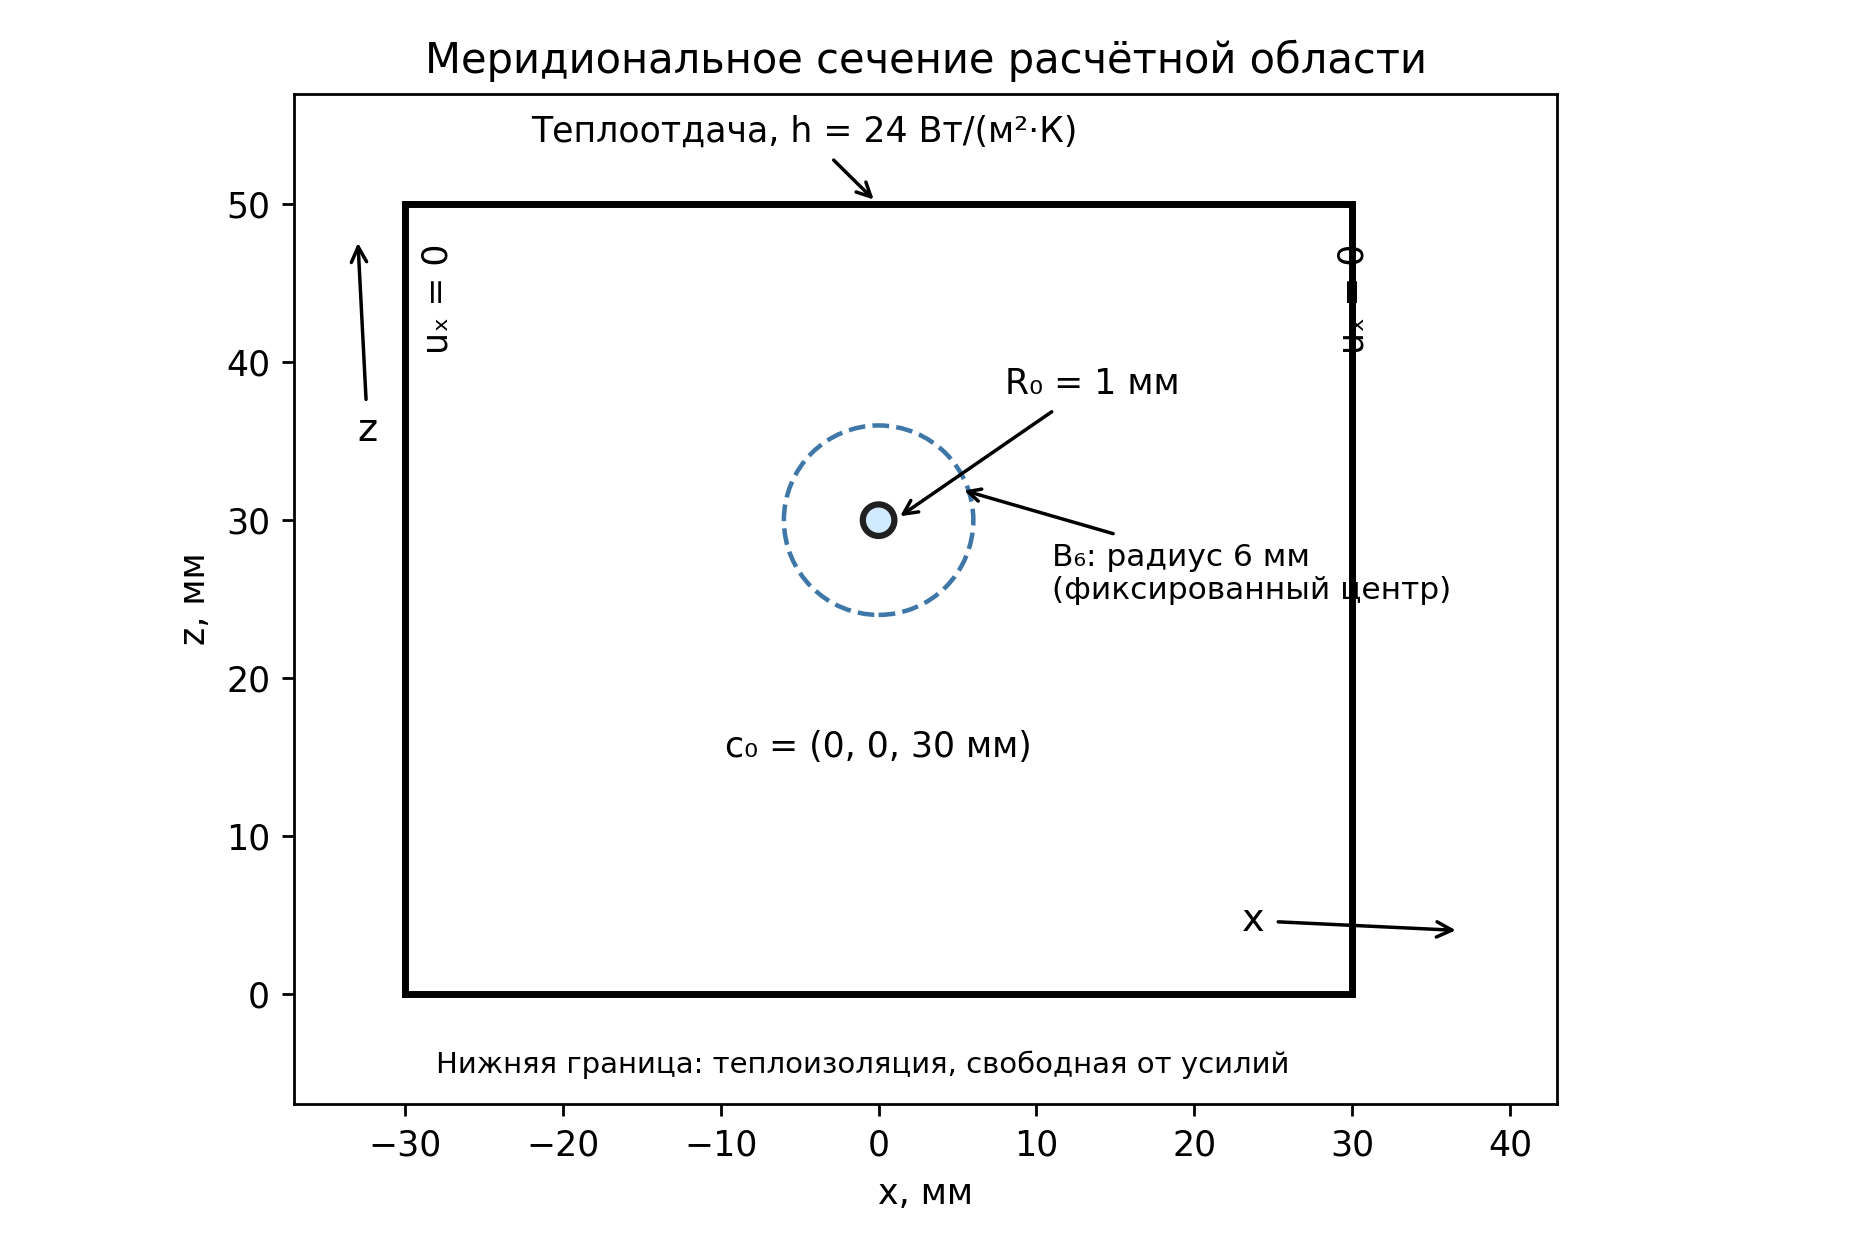
\includegraphics[width=13cm,height=\textheight]{fig1_geometry.png}
\caption{Меридиональное сечение фрагмента льда и фиксированная область
наблюдения}
\end{figure}

\emph{Рис. 1. Геометрия расчётного фрагмента, положение сферической
полости и область наблюдения \(B_6\) (схема в сечении \(xz\)). На гранях
\(y=\pm30\) мм также задано условие \(u_y=0\).}

В области \(\Omega\) решается нестационарное уравнение теплопроводности

\[
\rho c_p\,\frac{\partial T}{\partial t}-\nabla\!\cdot(k\nabla T)=0,\qquad T(\boldsymbol x,0)=T_0. \qquad(1)
\]

На верхней грани задано конвективное условие
\(-k\nabla T\cdot\boldsymbol n_{\Omega}=h(T-T_\infty)\), на остальных
внешних гранях и внутренней поверхности поры принят нулевой тепловой
поток. Температура окружающей среды имеет вид

\[
T_\infty(t,\xi)=T_0-\Delta T_0\,[1-\exp(-t/t_c)]+\sigma_\Theta\xi,\qquad \xi\sim N(0,1). \qquad(2)
\]

Случайная величина \(\xi\) фиксируется на протяжении одной временной
траектории. Это случайное смещение температурного уровня одной и той же
программы охлаждения, а не белый шум или независимые воздействия на
каждом временном шаге. Использованы \(T_0=253.15\) К, \(\Delta T_0=3\)
К, \(t_c=300\) с, \(\sigma_\Theta=0.48\) К, \(t_f=3600\) с,
\(\rho=920.3\) кг/м³, \(c_p=1960\) Дж/(кг·К), \(k=2.40\) Вт/(м·К),
\(h=24\) Вт/(м²·К). Воздух в полости не участвует в теплообмене; эффекты
конвекции и теплопроводности внутри неё исключены.

\subsection{3. Квазистатическая термомеханика и модель
материала}\label{ux43aux432ux430ux437ux438ux441ux442ux430ux442ux438ux447ux435ux441ux43aux430ux44f-ux442ux435ux440ux43cux43eux43cux435ux445ux430ux43dux438ux43aux430-ux438-ux43cux43eux434ux435ux43bux44c-ux43cux430ux442ux435ux440ux438ux430ux43bux430}

Для каждого температурного сценария рассматривается квазистатическое
равновесие

\[
-\nabla\cdot\boldsymbol\sigma=\boldsymbol0,\qquad
\boldsymbol\varepsilon=\tfrac12(\nabla\boldsymbol u+\nabla\boldsymbol u^{\mathsf T}),\qquad
\boldsymbol\varepsilon_T=\alpha(T-T_0)\boldsymbol I. \qquad(3)
\]

На гранях \(x=\pm30\) мм наложено \(u_x=0\), на \(y=\pm30\) мм ---
\(u_y=0\). Верхняя и нижняя грани, как и поверхность поры, свободны от
поверхностных сил. Неопределённость жёсткого вертикального переноса
устраняется условием \(\int_\Omega u_z\,dV=0\). Эти условия моделируют
горизонтально стеснённый фрагмент льда, но не бесконечную среду с
произвольно удалёнными границами.

Пусть \(\boldsymbol e=\boldsymbol\varepsilon-\boldsymbol\varepsilon_T\)
и
\(\boldsymbol e^{D}=\boldsymbol e-\tfrac13\operatorname{tr}(\boldsymbol e)\boldsymbol I\).
Приняты соотношения

\[
\boldsymbol\sigma=K_b(T)\operatorname{tr}(\boldsymbol e)\boldsymbol I+\boldsymbol s,\quad
\boldsymbol s=2G(T)(\boldsymbol e^{D}-\boldsymbol e_d-\boldsymbol e_v),\quad
G=\frac{E_{\mathrm{inst}}}{2(1+\nu)},\quad K_b=\frac{E_{\mathrm{inst}}}{3(1-2\nu)}. \qquad(4)
\]

Здесь \(\boldsymbol e_d\) и \(\boldsymbol e_v\) --- девиаторные
внутренние переменные запаздывающей и вязкой деформации, первоначально
равные нулю. Для модели EDV их кинетика определена следующим образом:

\[
\dot{\boldsymbol e}_d=A_d(T)\left[\frac32K_d\boldsymbol s-\boldsymbol e_d\right],\qquad
\dot{\boldsymbol e}_v=\frac32K_N(T)q^{m-1}\boldsymbol s,\qquad
q=\sqrt{\frac32\boldsymbol s:\boldsymbol s}. \qquad(5)
\]

Температурные множители \(A_d(T)\) и \(K_N(T)\) задаются относительно
\(T_r=263.15\) К аррениусовским законом
\(A_{\mathrm{arr}}=\exp[-Q/R_g(1/T-1/T_r)]\). Параметры:
\(A_{d,r}=1.5\cdot10^{-3}\) с⁻¹, \(K_d=1.2\cdot10^{-3}\) МПа⁻¹,
\(K_{N,r}=2.56\cdot10^{-7}\) МПа⁻ᵐ·с⁻¹, \(m=3.1\), \(Q=66.9\) кДж/моль,
\(\nu=0.35\), \(\alpha=149\cdot10^{-6}/3\) К⁻¹. При вычислениях
используются единицы СИ с явным преобразованием материальных
коэффициентов, заданных исходно в МПа.

Для мгновенного модуля использована нормировка относительной
температурной зависимости из {[}1{]}:

\[
E_{\mathrm{inst}}(T)=E_{\mathrm{ref}}\,\frac{8.93-0.012T_C}{9.17},\qquad
E_{\mathrm{ref}}=9500\ \text{МПа},\quad T_C=T-273.15. \qquad(6)
\]

Абсолютный уровень \(E_{\mathrm{ref}}\) является условным параметром
рассматриваемого материала, а не универсальной измеренной константой
пресноводного льда. Относительное изменение мгновенного модуля в
рассматриваемом узком температурном диапазоне и накопление внутренних
деформаций EDV физически разделены. Температура влияет на механическое
состояние; обратное тепловыделение от механической диссипации в (1) не
включено.

\subsection{4. Показатель растягивающего состояния и его геометрическая
чувствительность}\label{ux43fux43eux43aux430ux437ux430ux442ux435ux43bux44c-ux440ux430ux441ux442ux44fux433ux438ux432ux430ux44eux449ux435ux433ux43e-ux441ux43eux441ux442ux43eux44fux43dux438ux44f-ux438-ux435ux433ux43e-ux433ux435ux43eux43cux435ux442ux440ux438ux447ux435ux441ux43aux430ux44f-ux447ux443ux432ux441ux442ux432ux438ux442ux435ux43bux44cux43dux43eux441ux442ux44c}

Пусть \(\sigma_1\ge\sigma_2\ge\sigma_3\) --- главные значения полного
тензора напряжений. Введены фиксированный масштаб
\(\sigma_{\mathrm{ref}}=E_{\mathrm{ref}}\alpha\Delta T_0/(1-\nu)\),
безразмерные величины \(r_a=\sigma_a/\sigma_{\mathrm{ref}}\) и
сглаженная положительная часть
\(p_\epsilon(r)=[r+\sqrt{r^2+\epsilon_s^2}]/2\), где
\(\epsilon_s=10^{-3}\). Рассматриваемая спектральная функция имеет вид

\[
\Psi(\boldsymbol\sigma)=\sum_{a=1}^{3}p_\epsilon(r_a)^2. \qquad(7)
\]

Она гладко учитывает растягивающие главные напряжения; её значение не
является пределом прочности, критерием роста трещины либо вероятностью
разрушения. При нулевых напряжениях \(\Psi=7.5\cdot10^{-7}\) из-за
регуляризации.

Основная область наблюдения \(\Omega_6=\Omega\cap B_6\), где
\(B_6=\{\boldsymbol x:|\boldsymbol x-\boldsymbol c_0|<6R_0\}\) и
\(\boldsymbol c_0\) --- \textbf{исходный неизменяемый} центр. При
перемещении полости область \(B_6\) не переносится вместе с ней.
Определим

\[
\Phi_6(t,\xi)=\frac{1}{|\Omega_6|}\int_{\Omega_6}\Psi(\boldsymbol\sigma(\boldsymbol x,t,\xi))\,dV,
\qquad j_6(\xi)=\frac{1}{t_f}\int_0^{t_f}\Phi_6(t,\xi)\,dt. \qquad(8)
\]

В вычислительной реализации временной интеграл вычисляется
трапецеидальным правилом. Нормирование на изменяющийся объём
\(|\Omega_6|\) важно при вариациях формы; если
\(V_n=\boldsymbol V\cdot\boldsymbol n_c\) положительно, то
\(|\Omega_6|'[\boldsymbol V]=-\int_{\Gamma_c}V_n\,dS\) при малых
возмущениях внутри \(B_6\).

Геометрия поры возмущается тремя однопараметрическими семействами:
радиальное изменение \(R\), перенос \(t_z\) и нормальное смещение по
сферической гармонике \(Y_{20}\). Угловая функция при обычной
\(L^2(S^2)\)-нормировке равна

\[
Y_{20}(\theta)=\sqrt{\frac{5}{16\pi}}\,(3\cos^2\theta-1),\quad
V_n^{(R)}=1,\quad V_n^{(t_z)}=\cos\theta,\quad V_n^{(y20)}=Y_{20}(\theta). \qquad(9)
\]

Значения производных рассчитываются центральной конечной разностью по
соответствующему \textbf{размерному} параметру \(a\):

\[
D_a j_6(\xi)\approx\frac{j_6(a+\delta,\xi)-j_6(a-\delta,\xi)}{2\delta},\qquad \delta=5\cdot10^{-6}\ \text{м}. \qquad(10)
\]

В отличие от параметра \(t_z\), обозначающего перенос центра, \(y20\) в
этой формуле --- амплитуда нормального смещения в метрах, умноженная на
нормированную гармонику. Все три производные имеют размерность м⁻¹. В
частности, их абсолютные значения нельзя интерпретировать как
чувствительности к одинаковым относительным изменениям формы без
соответствующей нормировки.

\subsection{5. Случайное охлаждение и низкомодовое поле на поверхности
поры}\label{ux441ux43bux443ux447ux430ux439ux43dux43eux435-ux43eux445ux43bux430ux436ux434ux435ux43dux438ux435-ux438-ux43dux438ux437ux43aux43eux43cux43eux434ux43eux432ux43eux435-ux43fux43eux43bux435-ux43dux430-ux43fux43eux432ux435ux440ux445ux43dux43eux441ux442ux438-ux43fux43eux440ux44b}

Для стандартной нормальной случайной переменной \(\xi\) математическое
ожидание и дисперсия функционала определены равенствами

\[
M=\mathbb E[j_6],\qquad V=\mathbb E[(j_6-M)^2]. \qquad(11)
\]

В GH3 использованы узлы \(\xi_k=\{-\sqrt3,0,\sqrt3\}\) и веса
\(w_k=\{1/6,2/3,1/6\}\). В контрольной GH5 использованы узлы \(0\),
\(\pm1.35562618\), \(\pm2.85697001\) с весами соответственно
\(0.53333333\), \(0.22207592\) и \(0.01125741\) на каждый симметричный
узел. Производные моментов при фиксированной мере распределения имеют
вид

\[
D_aM=\sum_kw_kD_aj_k,\qquad
D_aV=2\sum_kw_k(j_k-M)D_aj_k. \qquad(12)
\]

Обратный знак нормали ледяной области на поверхности поры учитывается
через выбранную ориентацию \(\boldsymbol n_c\). Если существует
поверхностная плотность \(g_F\) производной формы для \(F=M\) или \(V\),
то

\[
D F[\boldsymbol V]=\int_{\Gamma_c}g_F V_n\,dS. \qquad(13)
\]

Поскольку в данном этапе вычислены лишь три модальные производные,
восстановить полный \(g_F(\theta,\varphi)\) нельзя. Используется его
ортогональная низкомодовая проекция:

\[
g_F^{(3)}(\theta)=\frac{D_RF}{4\pi R_0^2}
+\frac{3D_{t_z}F}{4\pi R_0^2}\cos\theta
+\frac{D_{y20}F}{R_0^2}Y_{20}(\theta). \qquad(14)
\]

При такой нормировке интегралы \(\int_{\Gamma_c}g_F^{(3)}\,dS\),
\(\int_{\Gamma_c}g_F^{(3)}\cos\theta\,dS\) и
\(\int_{\Gamma_c}g_F^{(3)}Y_{20}\,dS\) в точности воспроизводят исходные
модальные производные. При этом никаких сведений о гармониках более
высоких порядков из этих трёх интегралов не следует.

\subsection{6. Метод конечных элементов и
проверки}\label{ux43cux435ux442ux43eux434-ux43aux43eux43dux435ux447ux43dux44bux445-ux44dux43bux435ux43cux435ux43dux442ux43eux432-ux438-ux43fux440ux43eux432ux435ux440ux43aux438}

Трёхмерная область аппроксимировалась криволинейными квадратичными
тетраэдрами Tet10. В каждом температурном сценарии сначала решалась
тепловая задача, затем последовательность нелинейных задач механического
равновесия с обновлением внутренних переменных EDV. Для расчёта \(\Psi\)
используются три главных напряжения в точках интегрирования; объёмный
функционал осредняется по принятому приближению области \(\Omega_6\).
Пространственные интегралы вычислялись по трёхточечной квадратуре на
тетраэдре, обозначенной в расчётных протоколах как \texttt{q3}; она
\textbf{не совпадает} со стохастической квадратурой GH3. При вычислении
производных на \(+\delta\) и \(-\delta\) все физические параметры и узлы
случайной квадратуры сохранялись неизменными.

Сначала оценивались производные при \(\xi=0\) для девяти мод, включая
радиальное изменение, три переноса и пять квадрупольных гармоник. Затем
для трёх допускающих ненулевой отклик мод \(R\), \(t_z\), \(Y_{20}\)
вычислены производные ожидания и дисперсии на сетках H0, H2, H3 и H4. На
более тонких сетках выборочно проверены геометрический и временной шаги;
на H2 сравнивались GH3 и GH5. Данные исходных локальных FEM-траекторий
повторно не рассчитывались, если результаты уже сохранялись и могли
пройти проверку совместимости.

Проведённые проверки подтверждают внутреннюю арифметическую
согласованность стохастических таблиц и воспроизводимость расчётов по
конечным разностям. Они \textbf{не являются} независимым доказательством
малой ошибки линейных/нелинейных итераций вблизи симметрийных нулей,
равно как и доказательством сходимости к непрерывному градиенту формы.

\subsection{7. Результаты численного
исследования}\label{ux440ux435ux437ux443ux43bux44cux442ux430ux442ux44b-ux447ux438ux441ux43bux435ux43dux43dux43eux433ux43e-ux438ux441ux441ux43bux435ux434ux43eux432ux430ux43dux438ux44f}

\subsubsection{7.1. Геометрические производные при детерминированном
охлаждении}\label{ux433ux435ux43eux43cux435ux442ux440ux438ux447ux435ux441ux43aux438ux435-ux43fux440ux43eux438ux437ux432ux43eux434ux43dux44bux435-ux43fux440ux438-ux434ux435ux442ux435ux440ux43cux438ux43dux438ux440ux43eux432ux430ux43dux43dux43eux43c-ux43eux445ux43bux430ux436ux434ux435ux43dux438ux438}

Для \(\xi=0\) производные по радиусу, вертикальному перемещению и
\(Y_{20}\) на наиболее тонких использованных сетках соответственно
составили \(0.0971812\), \(-0.000509056\) и \(-0.0261417\) м⁻¹.
Радиальная производная первоначального детерминированного исследования
получена при \(\Delta t=150\) с, две другие --- при \(\Delta t=300\) с;
поэтому этот набор нельзя использовать для чистой оценки разности только
по геометрической моде при строго одинаковой временной схеме. В
последующей стохастической кампании все три моды рассчитаны совместно на
H4 при \(\Delta t=300\) с.

Для переносов \(t_x,t_y\) и неосесимметричных квадрупольных гармоник
\(Y_{21c},Y_{21s},Y_{22c},Y_{22s}\) непрерывная симметричная модель
предписывает нулевую первую вариацию. Дискретные результаты имели малые
ненулевые значения, уменьшающиеся при сгущении сетки для исследованных
мод. Эти остатки характеризуют численную асимметрию и погрешности
решения; приводить их как ненулевую физическую чувствительность было бы
некорректно.

\subsubsection{7.2. Случайное охлаждение: производные ожидания и
дисперсии}\label{ux441ux43bux443ux447ux430ux439ux43dux43eux435-ux43eux445ux43bux430ux436ux434ux435ux43dux438ux435-ux43fux440ux43eux438ux437ux432ux43eux434ux43dux44bux435-ux43eux436ux438ux434ux430ux43dux438ux44f-ux438-ux434ux438ux441ux43fux435ux440ux441ux438ux438}

На сетке H4 получены результаты, приведённые в табл. 1. Они относятся к
полной модели EDV с температурно-зависимым мгновенным модулем, шагом
\(\Delta t=300\) с и GH3.

\textbf{Таблица 1.} Производные моментов \(j_6\) по геометрическим
параметрам на H4.

\begin{longtable}[]{@{}
  >{\raggedright\arraybackslash}p{(\columnwidth - 6\tabcolsep) * \real{0.2500}}
  >{\raggedleft\arraybackslash}p{(\columnwidth - 6\tabcolsep) * \real{0.2500}}
  >{\raggedleft\arraybackslash}p{(\columnwidth - 6\tabcolsep) * \real{0.2500}}
  >{\raggedleft\arraybackslash}p{(\columnwidth - 6\tabcolsep) * \real{0.2500}}@{}}
\toprule\noalign{}
\begin{minipage}[b]{\linewidth}\raggedright
Мода
\end{minipage} & \begin{minipage}[b]{\linewidth}\raggedleft
\(D_aM\), м⁻¹
\end{minipage} & \begin{minipage}[b]{\linewidth}\raggedleft
\(D_aV\), м⁻¹
\end{minipage} & \begin{minipage}[b]{\linewidth}\raggedleft
\(D_aj_6(0)\), м⁻¹
\end{minipage} \\
\midrule\noalign{}
\endhead
\bottomrule\noalign{}
\endlastfoot
\(R\) & \(+0.100353733\) & \(+2.01428682\cdot10^{-4}\) &
\(+0.097210406\) \\
\(t_z\) & \(-0.000527234\) & \(-1.07481338\cdot10^{-6}\) &
\(-0.000509056\) \\
\(Y_{20}\) & \(-0.027015092\) & \(-5.46217171\cdot10^{-5}\) &
\(-0.026141658\) \\
\end{longtable}

Для исходной геометрии стохастическое среднее \(M\simeq0.0085752\),
дисперсия \(V\simeq8.6726\cdot10^{-6}\); коэффициент вариации составляет
около \(34.3\%\). Необходимо подчеркнуть, что это изменчивость
\textbf{безразмерного функционала напряжённого состояния}, а не
вероятность разрушения поры.

Радиальное увеличение повышает математическое ожидание и дисперсию
\(j_6\). Положительное вертикальное перемещение центра и положительная
амплитуда \(Y_{20}\) уменьшают оба момента при принятой ориентации
геометрического возмущения. По абсолютным размерным производным нельзя
непосредственно ранжировать практическую значимость мод, потому что
\(V_n^{(R)}=1\), \(V_n^{(t_z)}=\cos\theta\), а \(V_n^{(y20)}=Y_{20}\)
имеют разные нормировки. Нормированные значения \(S_a^M=(R_0/M)D_aM\)
составляют ориентировочно \(S_R^M=0.01170\), \(S_{t_z}^M=-0.0000615\),
\(S_{y20}^M=-0.00315\) для принятых амплитуд размерных геометрических
параметров. Такая запись характеризует изменение среднего при приращении
параметра на одну долю базового радиуса, а не локальное значение поля
напряжений.

\subsubsection{7.3. Сгущение пространственной
сетки}\label{ux441ux433ux443ux449ux435ux43dux438ux435-ux43fux440ux43eux441ux442ux440ux430ux43dux441ux442ux432ux435ux43dux43dux43eux439-ux441ux435ux442ux43aux438}

При переходе от H3 к H4 изменения модулей производных математического
ожидания составили \(0.196\%\) для \(R\), \(0.319\%\) для \(t_z\) и
\(1.042\%\) для \(Y_{20}\). Для производных дисперсии соответствующие
изменения равны \(0.197\%\), \(0.224\%\) и \(1.000\%\). Ранние переходы
H0→H2 и H2→H3 вызывали большие расхождения. Следовательно, три основные
производные демонстрируют пространственную стабилизацию, наиболее
выраженную для радиальной моды.

\begin{figure}
\centering
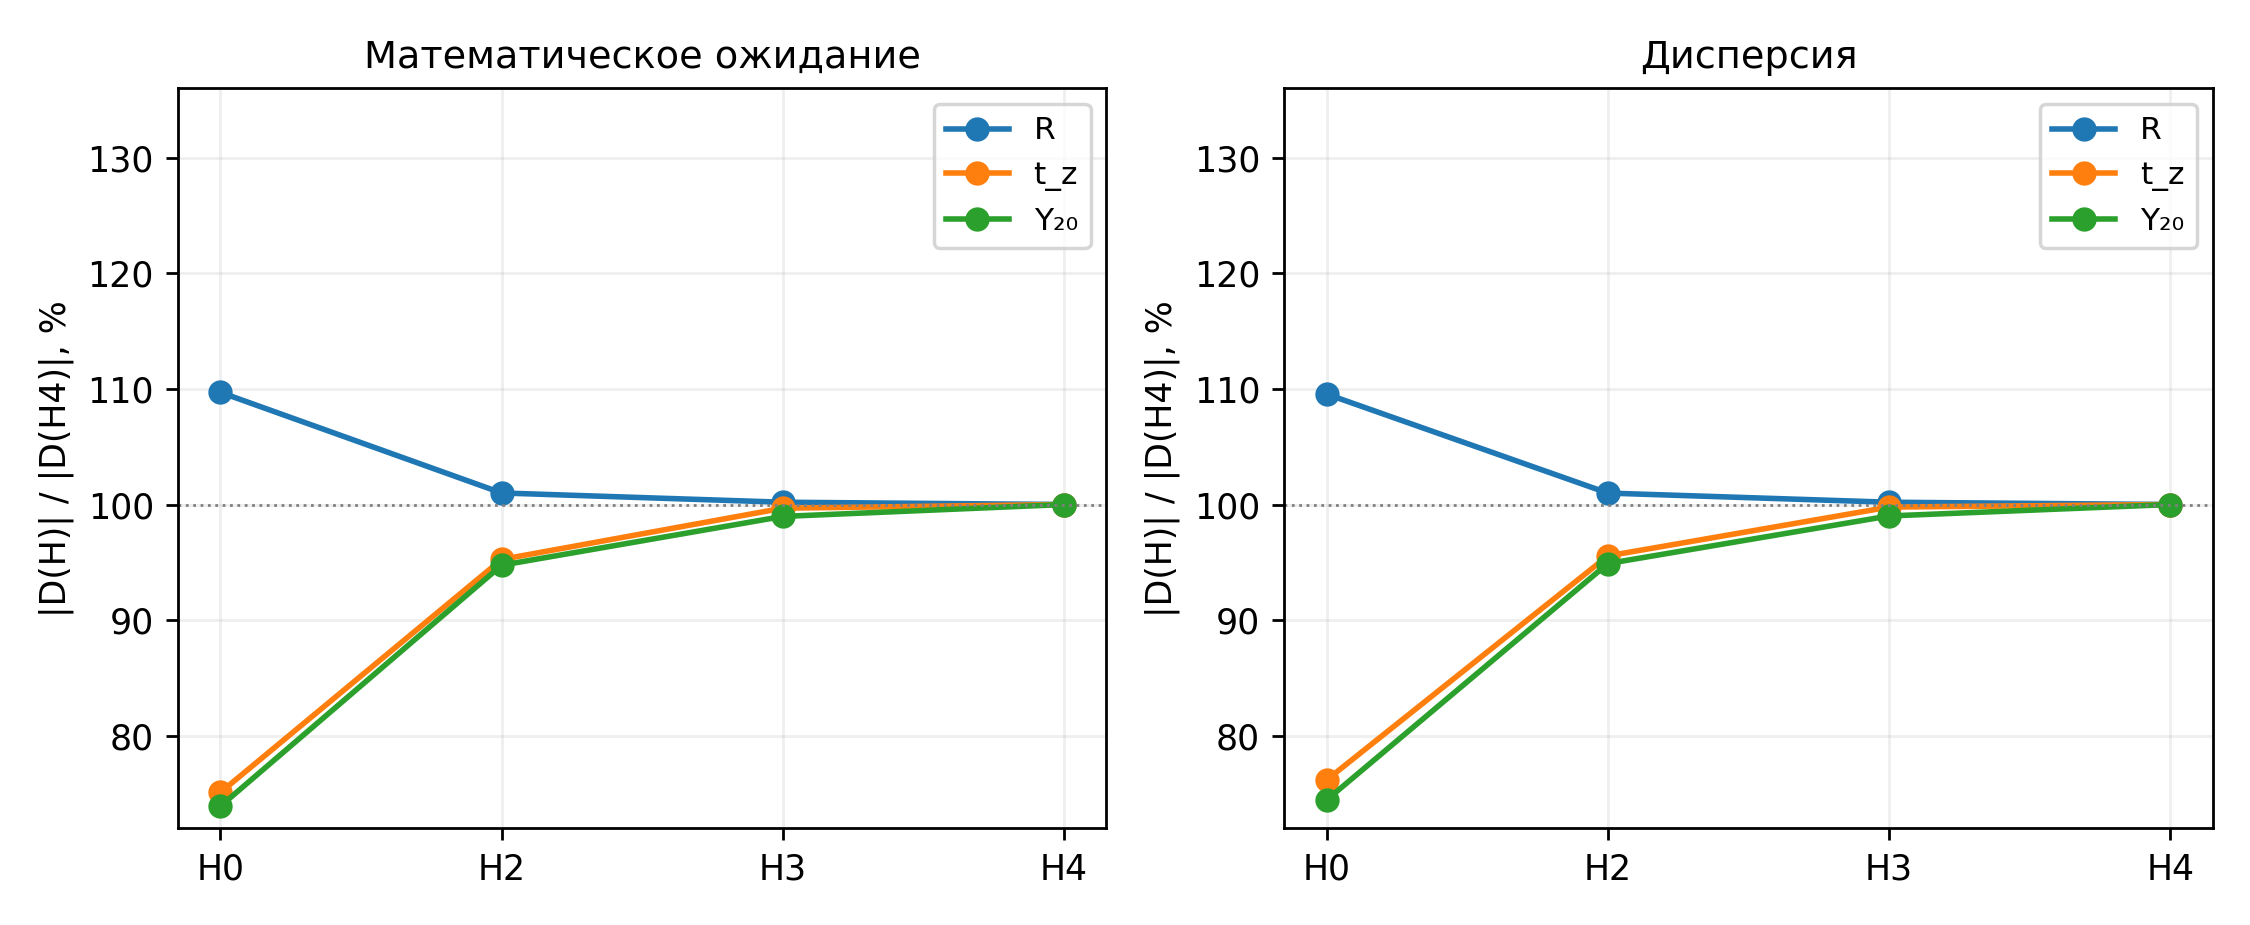
\includegraphics[width=15cm,height=\textheight]{fig2_spatial_convergence.png}
\caption{Пространственная стабилизация модальных производных ожидания и
дисперсии}
\end{figure}

\emph{Рис. 2. Отношения модулей производных на H0, H2, H3 к значениям H4
(100\%). В каждой моде нормирование производится отдельно. Сходимость
последовательности дискретных результатов не эквивалентна строгой оценке
ошибки непрерывной производной.}

\subsubsection{7.4. Изополя низкомодовой
чувствительности}\label{ux438ux437ux43eux43fux43eux43bux44f-ux43dux438ux437ux43aux43eux43cux43eux434ux43eux432ux43eux439-ux447ux443ux432ux441ux442ux432ux438ux442ux435ux43bux44cux43dux43eux441ux442ux438}

Подстановка данных табл. 1 в (14) даёт осесимметричные поля
\(g_M^{(3)}\) и \(g_V^{(3)}\). Для ожидания в верхнем полюсе,
экваториальной плоскости и нижнем полюсе получены соответственно
\(-9180.6\), \(+16506.2\), \(-8928.9\) м⁻³; для дисперсии ---
\(-18.6819\), \(+33.2564\), \(-18.1687\) м⁻³. Полученное поле
характеризуется положительным экваториальным поясом и отрицательными
полярными областями; небольшая асимметрия полюсов связана с вкладом
переноса \(t_z\).

\begin{figure}
\centering
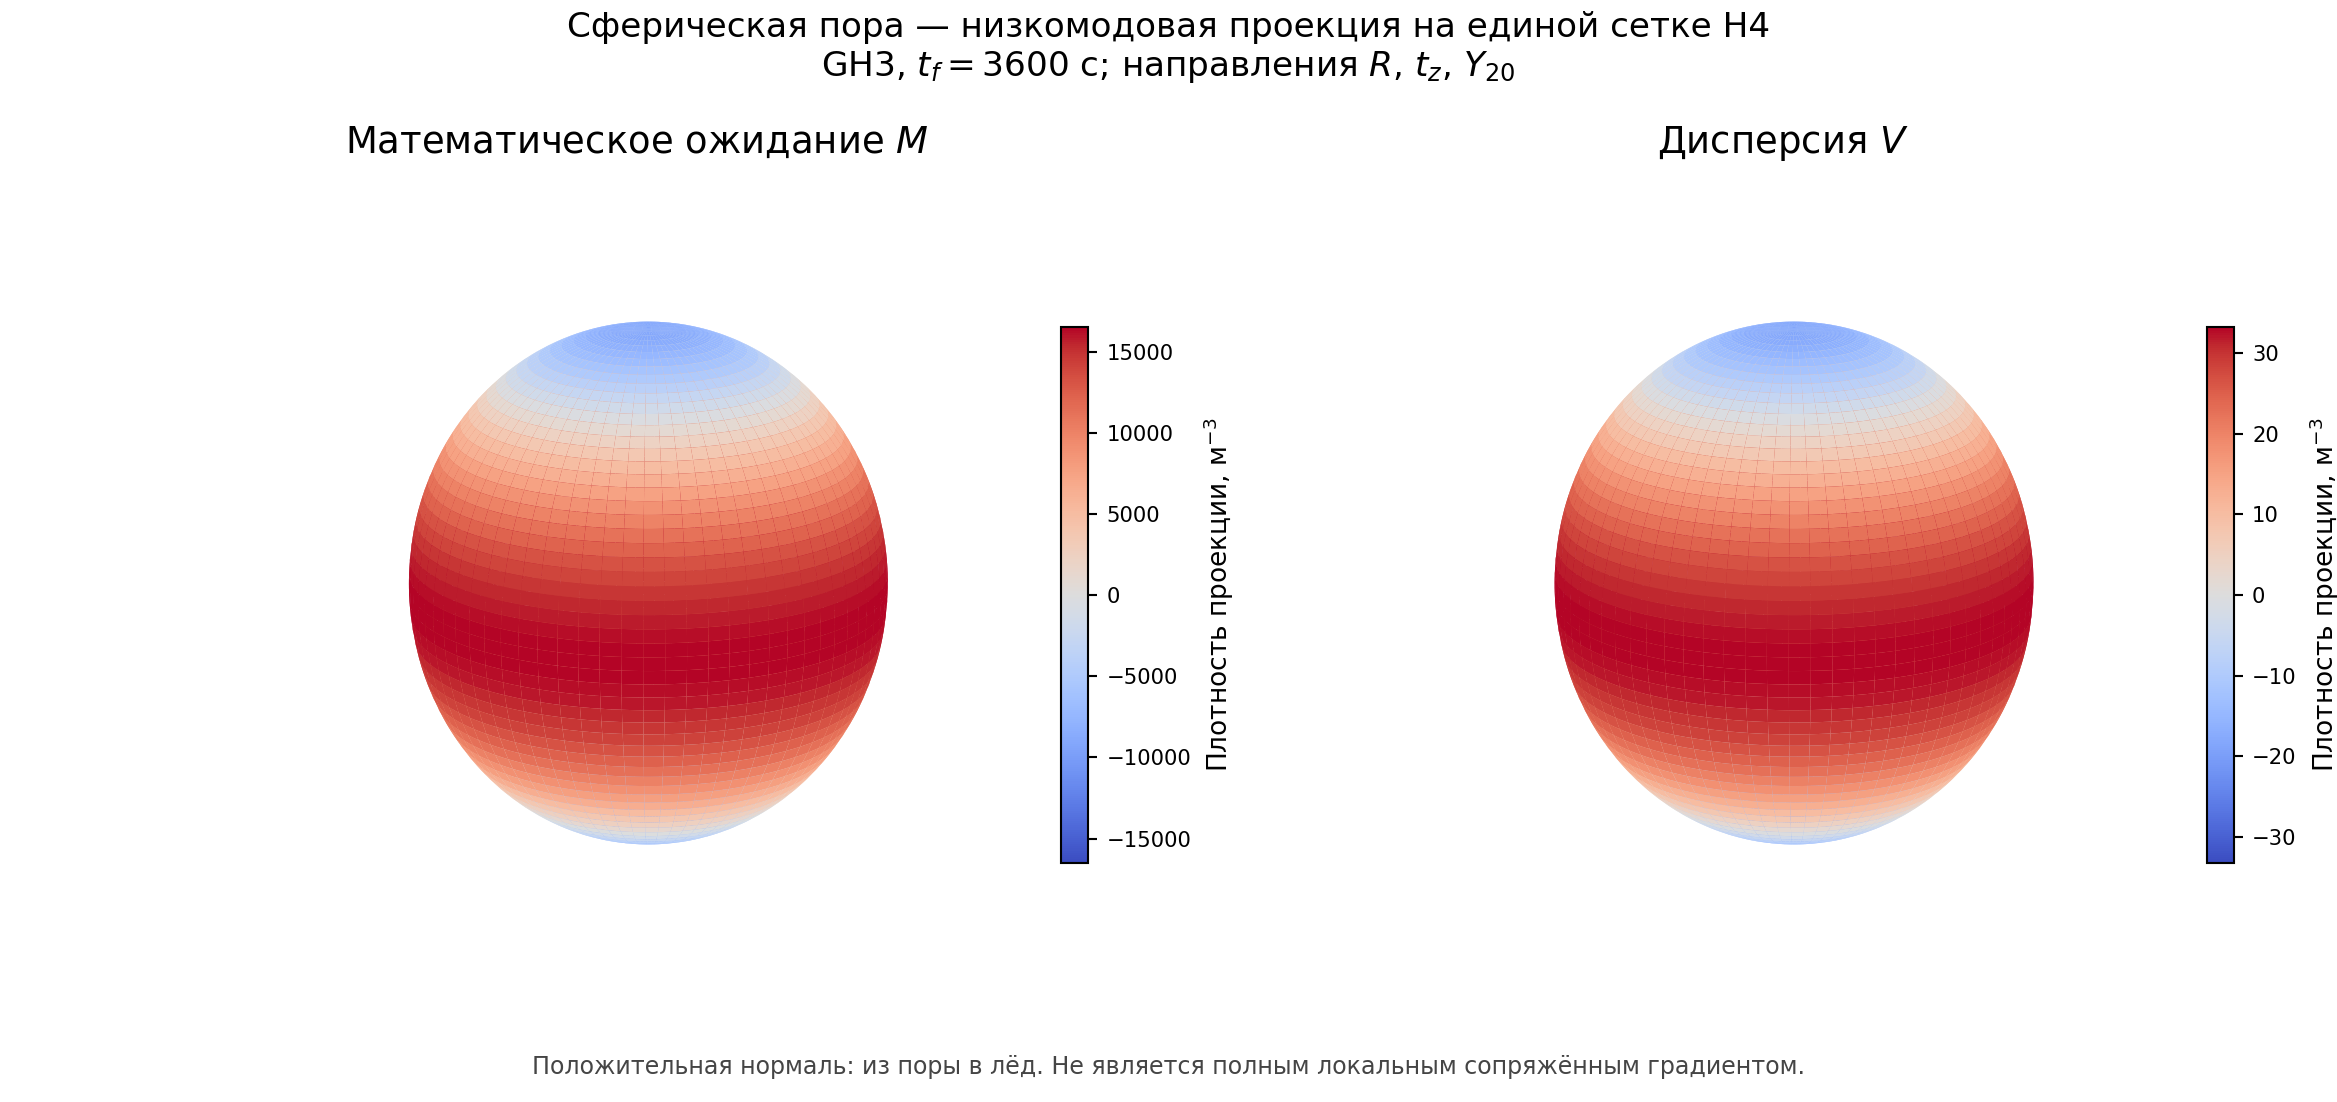
\includegraphics[width=15cm,height=\textheight]{fig3_modal_spheres.png}
\caption{Осесимметричные проекции плотности чувствительности для
моментов функционала}
\end{figure}

\emph{Рис. 3. Низкомодовые H4-проекции плотностей \(g_M^{(3)}\) (слева)
и \(g_V^{(3)}\) (справа) на поверхности сферической полости; нормаль
направлена от полости в лёд. Представленные поля не следует
отождествлять ни с точным локальным градиентом формы, ни с
распределением напряжений.}

Межсеточное изменение низкомодовых карт H3→H4 в относительной
поверхностной норме \(L^2\) равно примерно \(0.73\%\) для ожидания и
\(0.70\%\) для дисперсии. Интегрирование построенных полей по трём
исходным нормальным модам воспроизводит табличные производные с
относительным расхождением меньше \(10^{-8}\). Этот тест проверяет
\textbf{алгебру проекции}, а не наличие или отсутствие вклада высших
сферических гармоник.

\subsubsection{7.5. Шаг геометрического
возмущения}\label{ux448ux430ux433-ux433ux435ux43eux43cux435ux442ux440ux438ux447ux435ux441ux43aux43eux433ux43e-ux432ux43eux437ux43cux443ux449ux435ux43dux438ux44f}

Для моды \(Y_{20}\) на сетке H3 получены результаты при \(\delta=5\) и
\(10\) мкм. Производная ожидания изменилась на \(0.00378\%\), дисперсии
--- на \(0.00374\%\). Из-за квадратичной формальной ошибки центральной
разности можно построить условную экстраполяцию
\(D_0\approx(4D_5-D_{10})/3\); однако двух амплитуд недостаточно для
независимой проверки ожидаемого асимптотического порядка. Обнаруженное
влияние геометрического шага значительно меньше ранее выявленного
пространственного расхождения H3→H4 для \(Y_{20}\).

\subsubsection{7.6. Временная
дискретизация}\label{ux432ux440ux435ux43cux435ux43dux43dux430ux44f-ux434ux438ux441ux43aux440ux435ux442ux438ux437ux430ux446ux438ux44f}

Для \(Y_{20}\) на H3 сравнивались \(\Delta t=300,150,75,50\) с.
Результаты сведены в табл. 2.

\textbf{Таблица 2.} Временная сходимость производных на H3, \(Y_{20}\),
GH3.

\begin{longtable}[]{@{}rrr@{}}
\toprule\noalign{}
\(\Delta t\), с & \(D_{y20}M\), м⁻¹ & \(D_{y20}V\), м⁻¹ \\
\midrule\noalign{}
\endhead
\bottomrule\noalign{}
\endlastfoot
300 & \(-0.0267363862\) & \(-5.4080833\cdot10^{-5}\) \\
150 & \(-0.0267650775\) & \(-5.5209096\cdot10^{-5}\) \\
75 & \(-0.0267456916\) & \(-5.5672803\cdot10^{-5}\) \\
50 & \(-0.0267344401\) & \(-5.5809297\cdot10^{-5}\) \\
\end{longtable}

\begin{figure}
\centering
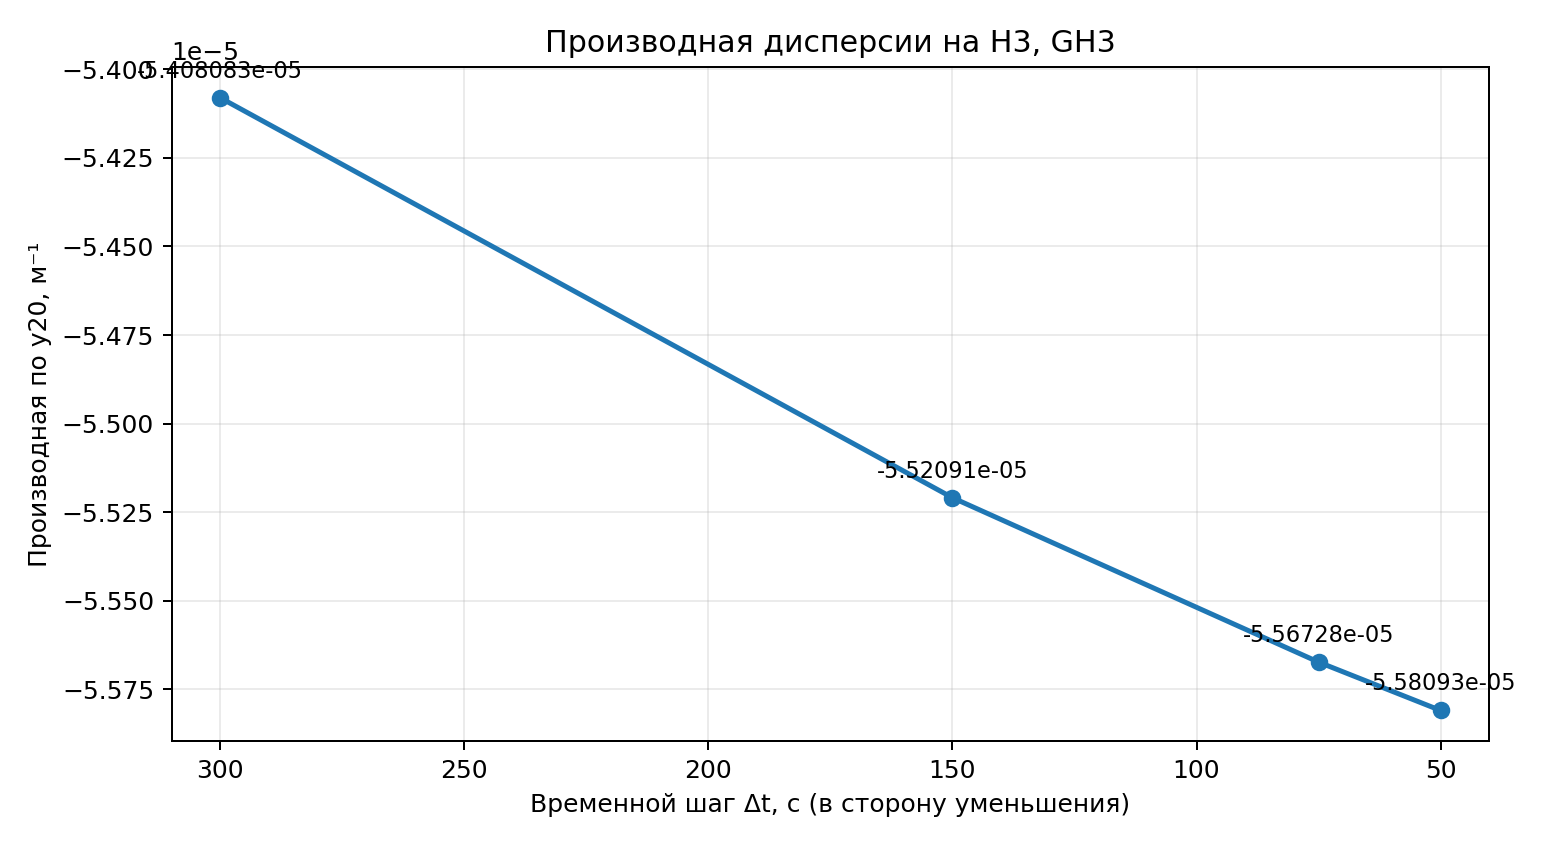
\includegraphics[width=13cm,height=\textheight]{fig4_temporal.png}
\caption{Временная сходимость производной дисперсии}
\end{figure}

\emph{Рис. 4. Изменение производной дисперсии по \(Y_{20}\) на H3 при
уменьшении временного шага.}

Производная ожидания изменяется немонотонно; при переходе 75→50 с
отличие по модулю равно \(0.042\%\). Производная дисперсии демонстрирует
более регулярную тенденцию, но сильнее зависит от шага: от 300 до 50 с
её модуль увеличивается примерно на \(3.20\%\), а при последнем переходе
--- на \(0.245\%\). Условные экстраполяции по двум тройкам шагов дают
предел около \(-5.60\cdot10^{-5}\) м⁻¹. Они основаны на предположении
степенного закона ошибки и не являются строгой апостериорной оценкой.

Следовательно, малая ошибка среднего не гарантирует малую ошибку
дисперсии. Односеточная H4-карта построена при 300 с, тогда как контроль
времени выполнен для H3. Это ограничивает возможные утверждения о её
окончательной количественной точности.

\subsubsection{7.7. Проверка квадратуры
Гаусса--Эрмита}\label{ux43fux440ux43eux432ux435ux440ux43aux430-ux43aux432ux430ux434ux440ux430ux442ux443ux440ux44b-ux433ux430ux443ux441ux441ux430ux44dux440ux43cux438ux442ux430}

На H2 при \(\Delta t=300\) с для \(Y_{20}\) проведено контролируемое
сравнение GH3 и GH5. В последней реализации сохранённые совместимые
траектории \(\xi=0\) использовались повторно. Получены изменения
производной ожидания менее \(10^{-6}\%\) и производной дисперсии порядка
\(0.00035\%\) (табл. 3). Это существенно меньше наблюдавшихся
пространственных и временных изменений.

\textbf{Таблица 3.} Влияние порядка вероятностной квадратуры на H2,
\(Y_{20}\).

\begin{longtable}[]{@{}
  >{\raggedright\arraybackslash}p{(\columnwidth - 4\tabcolsep) * \real{0.3333}}
  >{\raggedleft\arraybackslash}p{(\columnwidth - 4\tabcolsep) * \real{0.3333}}
  >{\raggedleft\arraybackslash}p{(\columnwidth - 4\tabcolsep) * \real{0.3333}}@{}}
\toprule\noalign{}
\begin{minipage}[b]{\linewidth}\raggedright
Характеристика
\end{minipage} & \begin{minipage}[b]{\linewidth}\raggedleft
GH3
\end{minipage} & \begin{minipage}[b]{\linewidth}\raggedleft
GH5
\end{minipage} \\
\midrule\noalign{}
\endhead
\bottomrule\noalign{}
\endlastfoot
\(M\) & \(0.008576832188\) & \(0.008576832224\) \\
\(V\) & \(8.67585404\cdot10^{-6}\) & \(8.67588427\cdot10^{-6}\) \\
\(D_{y20}M\), м⁻¹ & \(-0.025596411196\) & \(-0.025596411324\) \\
\(D_{y20}V\), м⁻¹ & \(-5.18321047\cdot10^{-5}\) &
\(-5.18322840\cdot10^{-5}\) \\
\end{longtable}

Таким образом, для проверенной конфигурации GH3 практически
воспроизводит GH5. Распространять это утверждение на все значения
температуры, геометрии и временных шагов без дальнейших расчётов не
следует.

\subsection{8. Обсуждение результатов и
ограничения}\label{ux43eux431ux441ux443ux436ux434ux435ux43dux438ux435-ux440ux435ux437ux443ux43bux44cux442ux430ux442ux43eux432-ux438-ux43eux433ux440ux430ux43dux438ux447ux435ux43dux438ux44f}

Первый физический результат связан с различными знаками отклика на три
геометрические моды. Увеличение радиуса воздушного включения в
рассматриваемой модели повышает осреднённый показатель растягивающего
состояния и его дисперсию. Вертикальный перенос центра и положительное
возмущение \(Y_{20}\) изменяют оба момента в противоположную сторону.
Вследствие малого значения производной по вертикальному переносу особую
важность приобретает раздельный контроль абсолютной погрешности и
симметрийных нулей.

Второй результат состоит в непрямой связи между стохастической
изменчивостью функционала и производными его моментов. При изменении
временного шага среднее \(j_6\) и его производная ведут себя существенно
устойчивее, чем дисперсия и её производная. Поэтому проверка только
детерминированного узла \(\xi=0\) или только среднего функционала
недостаточна для количественного описания геометрической
чувствительности дисперсии.

Третий результат представляет построение низкомодовой поверхностной
карты. Установленный контраст экваториальной области и полюсов следует
из сочетания радиальной, трансляционной и квадрупольной компонент.
Однако восстановленное поле ограничено линейной оболочкой \(1\),
\(\cos\theta\), \(Y_{20}\). В частности, даже если все три интегральные
производные вычислены с высокой точностью, могут существовать компоненты
истинного градиента, ортогональные этим функциям. Для физического
истолкования локальных максимумов необходим независимый сопряжённый или
иной полевой расчёт.

Основные ограничения настоящего этапа заключаются в следующем.
Рассматривается один класс геометрии и механического стеснения;
теплопроводность воздуха, внутреннее давление, анизотропия и образование
трещин исключены. Мгновенный модуль задан относительной температурной
зависимостью при условном абсолютном уровне; параметры не были
идентифицированы для конкретного ледяного образца. Наблюдаемая область
\(B_6\) фиксирована относительно исходного центра, а дискретный выбор
элементов этой области может вносить дополнительную негладкость
функционала при вариации геометрии. При этом полные парные расчёты
E/ED/EDV и \(E_{\mathrm{const}}/E_{\mathrm{var}}\), а также дискретный
сопряжённый градиент формы ещё не завершены. Поэтому в настоящей
редакции нельзя заявлять количественную оценку \textbf{вклада самой
вязкоупругой релаксации} относительно чисто упругой модели или точное
локальное распределение градиента формы.

\subsection{9.
Заключение}\label{ux437ux430ux43aux43bux44eux447ux435ux43dux438ux435}

Для трёхмерной модели пресноводного льда со сферической воздушной порой,
квазистатической механикой EDV и случайным поверхностным охлаждением
выполнена серия конечно-элементных расчётов геометрических производных
локального функционала \(j_6\). На сетке H4 получены положительные
производные ожидания и дисперсии по радиусу, отрицательные --- по
вертикальному переносу центра и по осесимметричной гармонике \(Y_{20}\).
Симметрийные моды, обязанные давать нуль в непрерывной постановке,
использованы как дополнительные тесты дискретного решения.

Результаты H3 и H4 демонстрируют пространственную стабилизацию трёх
ненулевых производных: межсеточные изменения составляют не более
примерно \(1.05\%\) для исследованных стохастических моментов. Удвоение
шага геометрического возмущения с 5 до 10 мкм практически не меняет
результат для \(Y_{20}\) на H3. В то же время проверка временной
дискретизации выявила повышенную чувствительность производной дисперсии:
уменьшение \(\Delta t\) с 300 до 50 с изменило её модуль примерно на
\(3.20\%\). Замена GH3 на GH5 на тестовой конфигурации H2 дала
значительно меньший эффект.

На основе трёх модальных производных построена низкомодовая
осесимметричная проекция поверхностной плотности первой вариации,
показывающая противоположные знаки полярного и экваториального вкладов.
Полученная карта является полезным интегральным представлением
чувствительности, но не заменяет точный локальный градиент формы.
Дальнейший этап состоит в дискретном сопряжённом дифференцировании
полной термомеханической истории и в количественном сравнении моделей
упругого, запаздывающего и вязкого деформирования при одинаковых
тепловых и геометрических условиях.

\subsection{Литература}\label{ux43bux438ux442ux435ux440ux430ux442ux443ux440ux430}

\begin{enumerate}
\def\labelenumi{\arabic{enumi}.}
\tightlist
\item
  Sinha N.K. Elasticity of natural types of polycrystalline ice // Cold
  Regions Science and Technology. 1989. Vol. 17, No.~2. P. 127--135.
  DOI: 10.1016/S0165-232X(89)80003-5.
\item
  Chang X., Liu W., Zuo G., Dou Y., Li Y. Research on ultrasonic-based
  investigation of mechanical properties of ice // Acta Oceanologica
  Sinica. 2021. Vol. 40, No.~10. P. 97--105. DOI:
  10.1007/s13131-021-1890-3.
\item
  Galadima Y.K., Oterkus E., Oterkus S. Peridynamic modelling of elastic
  and viscoelastic behaviour in polycrystalline ice: a study using
  NOSBPD and PDCHT // Ocean Engineering. 2024. Vol. 312. Art. 119241.
  DOI: 10.1016/j.oceaneng.2024.119241.
\item
  Sahragard F., Pouragha M., Rayhani M. Thermobarokinetics of ice:
  constitutive formulation for the coupled effect of temperature,
  stress, and strain rate in ice // The Cryosphere. 2026. Vol. 20. P.
  595--608. DOI: 10.5194/tc-20-595-2026.
\item
  Zenkour A.M., Mashat D.S., Allehaibi A.M. Magneto-Thermoelastic
  Response in an Unbounded Medium Containing a Spherical Hole via
  Multi-Time-Derivative Thermoelasticity Theories // Materials. 2022.
  Vol. 15, No.~7. Art. 2432. DOI: 10.3390/ma15072432.
\item
  Youssef H.M., Alghamdi A.A. Influence of the fractional-order strain
  on an infinite material with a spherical cavity under Green-Naghdi
  hyperbolic two-temperature thermoelasticity theory // Journal of
  Engineering and Thermal Sciences. 2023. Vol. 3, No.~1. P. 11--24. DOI:
  10.21595/jets.2023.23372.
\item
  Delfour M.C., Zolésio J.-P. Structure of shape derivatives for
  nonsmooth domains // Journal of Functional Analysis. 1992. Vol. 104,
  No.~1. P. 1--33. DOI: 10.1016/0022-1236(92)90087-Y.
\item
  Brügger R., Harbrecht H., Tausch J. On the numerical solution of a
  time-dependent shape optimization problem for the heat equation //
  SIAM Journal on Control and Optimization. 2021. Vol. 59, No.~2. P.
  931--953. DOI: 10.1137/19M1268628.
\item
  Baumann P., Sturm K. Adjoint-based methods to compute higher-order
  topological derivatives with an application to elasticity //
  Engineering Computations. 2022. Vol. 39, No.~1. P. 60--114. DOI:
  10.1108/EC-07-2021-0407.
\item
  Shahan J.T., Walker S.W. Exact shape derivatives with unfitted finite
  element methods // Journal of Numerical Mathematics. 2026. Vol. 34,
  No.~1. P. 91--124. DOI: 10.1515/jnma-2024-0113.
\item
  Xiu D., Hesthaven J.S. High-order collocation methods for differential
  equations with random inputs // SIAM Journal on Scientific Computing.
  2005. Vol. 27, No.~3. P. 1118--1139. DOI: 10.1137/040615201.
\end{enumerate}

\end{document}
